\documentclass[letterpaper,10pt]{article}
\usepackage[pdftex]{graphicx}
\usepackage{listings}
\usepackage{alltt}
\usepackage{color}
\usepackage{amsmath}
\usepackage{hyperref}
\usepackage{pgfplotstable}

\definecolor{dkgreen}{rgb}{0,0.6,0}
\definecolor{gray}{rgb}{0.5,0.5,0.5}
\definecolor{mauve}{rgb}{0.58,0,0.82}

\hypersetup{
    colorlinks,
    citecolor=black,
    filecolor=black,
    linkcolor=black,
    urlcolor=black
}

\lstset{
	basicstyle=\footnotesize,
	breaklines=true,
	 backgroundcolor=\color{white},   % choose the background color; you must add \usepackage{color} or \usepackage{xcolor}
  basicstyle=\footnotesize,        % the size of the fonts that are used for the code
  breakatwhitespace=false,         % sets if automatic breaks should only happen at whitespace
  breaklines=true,                 % sets automatic line breaking
  captionpos=b,                    % sets the caption-position to bottom
  commentstyle=\color{dkgreen},    % comment style
  deletekeywords={...},            % if you want to delete keywords from the given language
  escapeinside={\%*}{*)},          % if you want to add LaTeX within your code
  extendedchars=true,              % lets you use non-ASCII characters; for 8-bits encodings only, does not work with UTF-8
  frame=single,	                   % adds a frame around the code
  keepspaces=true,                 % keeps spaces in text, useful for keeping indentation of code (possibly needs columns=flexible)
  keywordstyle=\color{blue},       % keyword style
  otherkeywords={*,grep,sort,head,mv,perl,chmod,...},           % if you want to add more keywords to the set
  numbers=left,                    % where to put the line-numbers; possible values are (none, left, right)
  numbersep=5pt,                   % how far the line-numbers are from the code
  numberstyle=\tiny\color{gray}, % the style that is used for the line-numbers
  rulecolor=\color{black},         % if not set, the frame-color may be changed on line-breaks within not-black text (e.g. comments (green here))
  showspaces=false,                % show spaces everywhere adding particular underscores; it overrides 'showstringspaces'
  showstringspaces=false,          % underline spaces within strings only
  showtabs=false,                  % show tabs within strings adding particular underscores
  stepnumber=1,                    % the step between two line-numbers. If it's 1, each line will be numbered
  stringstyle=\color{mauve},     % string literal style
  tabsize=2,	                   % sets default tabsize to 2 spaces
  title=\lstname                   % show the filename of files included with \lstinputlisting; also try caption instead of title
}


\begin{document} 

\begin{titlepage}

\begin{center}

\Huge{Assignment 3}

\Large{CS532-s16:  Web Sciences}

\Large{Spring 2016}

\Large{John Berlin}

\Large Generated on \today

\end{center}

\end{titlepage}
\newpage
\section*{1}
\subsection*{Question}
\begin{verbatim}
 1.  Download the 1000 URIs from assignment #2.  "curl", "wget", or
"lynx" are all good candidate programs to use.  We want just the
raw HTML, not the images, stylesheets, etc.

from the command line:

% curl http://www.cnn.com/ > www.cnn.com

% wget -O www.cnn.com http://www.cnn.com/

% lynx -source http://www.cnn.com/ > www.cnn.com

"www.cnn.com" is just an example output file name, keep in mind
that the shell will not like some of the characters that can occur
in URIs (e.g., "?", "&").  You might want to hash the URIs, like:

% echo -n "http://www.cs.odu.edu/show_features.shtml?72" | md5
41d5f125d13b4bb554e6e31b6b591eeb

("md5sum" on some machines; note the "-n" in echo -- this removes
the trailing newline.) 

Now use a tool to remove (most) of the HTML markup.  "lynx" will
do a fair job:

% lynx -dump -force_html www.cnn.com > www.cnn.com.processed

Use another (better) tool if you know of one.  Keep both files 
for each URI (i.e., raw HTML and processed).
\end{verbatim}
\subsection*{Answer}

Downloading the \verb+URI's+ was relatively simple thanks to using shell scripts which can be
found in listing \ref{lst:getHTML}. The script takes no arguments as I wish to make things as fire and forget as possible. So make sure your in the working directory of all the files.  

To run the script execute it as such:
\begin{lstlisting}[frame=single]
$ chmod +x hashUrisDownload.sh
$ ./hashUrisDownload.sh
\end{lstlisting}


The process is described as such. See the comments in the listing for full details.
\begin{enumerate}
\item Get the working directory and make file structure
\item For each \verb+URI+ in thousand.dat downloaded the \verb+URI-R+ and gets its hash. Curl with a supplied user agent and md5sum are used to produce these results. I use awk to print only the hash produced by md5sum.  
\item Append the \verb+URI+ and its hash \verb+ulrToHash.csv+
\item Clean up after ourselves \verb+ulrToHash.csv+. To do so I use find with -size 0c. 0c means I want to find files that are 0 bytes or empty 
\end{enumerate}

To strip the html from the files I first used lynx but was extremely disappointed with it.
I found it to keep way too much of the javascript and style tag contents. A better method was hinted at thus I looked into it. Thanks to my favourite search engine \href{www.duckduckgo.com}{DuckDuckGo} I was directed to use this language called \verb+Perl+.

To run the script execute it as such:
\begin{lstlisting}[frame=single]
$ perl removeHtml.pl
\end{lstlisting}

The \verb+Perl+ script used to correctly remove the html content from the hash.html files is found in listing \ref{lst:nukeHTML}. The process in brief is as such. See the comments in the listing for full details.
\begin{enumerate}
\item Libraries 
\begin{enumerate}
\item File::Slurp read the entire file
\item HTML::Restrict restrict(remove) html elements from the dom. As indicated in the parentheses I use HTML::Restrict to remove all html elements entirely. Leaving only the true text contents behind
\item File::Basename I want only the basename of the file xyz not xyz.html
\item Cwd I need to know man where are we
\end{enumerate}
\item Get where we are currently and set variables to the expected directory structure
\item Create a new HTML::Restrict object with args setting extra tags to nuke and trim resulting naked dom
\item Strip the dom and create processed file
\end{enumerate}

\newpage
\lstinputlisting[language=sh,
frame=single,
caption={Download HTML shell script},label=lst:getHTML,captionpos=b]{hashUrisDownload.sh}

\lstinputlisting[language=Perl,
frame=single,
caption={Perl script to remove all html},label=lst:nukeHTML,captionpos=b]{removeHtml.pl}  
\newpage    
\section*{2}
\subsection*{Question}
\begin{verbatim}
2.  Choose a query term (e.g., "shadow") that is not a stop word
(see week 5 slides) and not HTML markup from step 1 (e.g., "http")
that matches at least 10 documents (hint: use "grep" on the processed
files).  If the term is present in more than 10 documents, choose
any 10 from your list.  (If you do not end up with a list of 10
URIs, you've done something wrong).

As per the example in the week 5 slides, compute TFIDF values for
the term in each of the 10 documents and create a table with the
TF, IDF, and TFIDF values, as well as the corresponding URIs.  The
URIs will be ranked in decreasing order by TFIDF values.  For
example:

Table 1. 10 Hits for the term "shadow", ranked by TFIDF.

TFIDF	TF	IDF	URI
-----	--	---	---
0.150	0.014	10.680	http://foo.com/
0.044	0.008	 5.510	http://bar.com/


You can use Google or Bing for the DF estimation.  To count the
number of words in the processed document (i.e., the deonminator
for TF), you can use "wc":

% wc -w www.cnn.com.processed
    2370 www.cnn.com.processed

It won't be completely accurate, but it will be probably be
consistently inaccurate across all files.  You can use more 
accurate methods if you'd like.  

Don't forget the log base 2 for IDF, and mind your significant
digits!
\end{verbatim}
\newpage
\subsection*{Answer}
The term I choose to search for was \emph{Bernie} as I mined Twitter for \verb+Uri's+ during a democratic debate. I did so by executing the following command in the processed directory created by listing \ref{lst:getHTML}: 
\begin{lstlisting}[frame=single,language=sh,label=lst:topten]
$ grep -wic "Bernie" *.processed | sed -r "s/([a-z0-9.]+)(:)([0-9]+)/\1 \3/g" | awk '{print $2" "$1}' | sort -rn | head -n 10 | awk '{print $2}' >> tenForTFID.txt
$ mv tenForTFID.txt ../ 
\end{lstlisting}

Before I begin explaining this wonderful little shell snippet, the snippet was derived from reading ``Linux Command Line and Shell Scripting Bible" \cite{linuxBible} and consulting the man pages.

\begin{enumerate}
\item grep: to search for Bernie in the files
\begin{enumerate}
\item w: select only lines containing matches that form whole words
\item i: ignore case
\item c: print only a count of matching lines
\end{enumerate}
\item sed: replace string in a stream
\begin{enumerate}
\item r: use extended regex
\item expression: match md5sum separator count and replace separator with space
\end{enumerate}
\item awk: swap position of output
\item sort: sort output numerically and reverse it(descending order)
\item head: take top n
\item awk: print only the md5sum
\item append to file 
\end{enumerate}


I executed the command with out appending the output to a file and here is the produced output:
\begin{lstlisting}[frame=single]
d632bfc8f91eae4cf2c82eb0fd91a7fd.processed
9e1da9cae84ac0736037f14dd0970dd0.processed
404f907cde379d931becd4a90beb842a.processed
60746a6ce366dc48267249969f1cc353.processed
29e1a6b7baf3b7072cfb3c2f36262f4d.processed
e9db1fa8fe181f0b4ee4f5ae446e1a27.processed
d0bea5f71f177067314bee1bc60b2ccb.processed
3d9f071482d0909d263b37e6dc9d6b35.processed
f58549dc1ceb8afb01a6fee5daa03e48.processed
e79dcc12c17c9ac0dc5a45ac9e0f80df.processed
\end{lstlisting}

These files are only the top ten files that contain the term ``Bernie" which are saved for later. Now to figuring out how to calculate \(TF\), \(IDF\), and \(TDIDF\) for these files.


We know that \(TF\) is calculated per document as: \[ TF(Bernie,doc)= \frac{termCount(Bernie,doc)}{wordCount(doc)} \]


For the \(IDF\) calculation we must first do some searching on the internet to find out how many pages Google has and how many results are returned to use for the term \emph{Bernie}. Google has roughly 49 billion web pages indexed according to \emph{worldwidewebsize}  \cite{wwwsize} and a search for \emph{Bernie} gives us $105,000,000$ results. 


Using those numbers we can do some plug and chug to determine our \(IDF\) value with consideration to the effect of significant digits for logs as described in ``
Significant Figure Rules for Logarithm" \cite{sigdig}.
\[ IDF = \log_2 \left( \frac{49,000,000,000}{105,000,000} \right)  = \log_2 (466.6666) =  8.866248
\] 

But lets just use 8.8662 as empirically you cant round up from 3 ;).

Using the \emph{IDF} value we can now state the formula for the \(TFIDF\) for each of our ten documents as:
\[ TFIDF(Bernie,doc) = TF(Bernie,doc) * 8.8662\]



Now that we have our calculations down how about generating the numbers. Once again I felt like taking the easy mode and created a shell script to do all the work for me as seen in listing \ref{lst:tfid}. Once again I direct you to view the comments in the file for further details into how it operates.

But in brief the scrip operates as such:
\begin{enumerate}
\item For each of the hashed uris in the \emph{tenForTFID.txt} file
\item Get the total word count for the file
\item Get the term count again for \emph{Bernie}
\item Calculate the TF, and TFIDF
\item Append the TF IDF TFIDF and URI to the file \emph{tfidftable.csv}
\end{enumerate}

The results dumped to the file \emph{tfidftable.csv} can be found in table \ref{table:tfidf}.


\newpage
\lstinputlisting[language=sh,
frame=single,
caption={Find the count and  TFID},label=lst:tfid,captionpos=b]{findten.sh}

\begin{table}
\begin{tabular}{ | l | l | l | p{8.0cm} | }
\hline
\textbf{TFIDF} & \textbf{IDF} & \textbf{TF} & \textbf{URI} \\
\hline
0.00153 & 8.8061 & 0.01347 &  \url{http://www.salon.com/2015/02/01/football_an_american_tragedy/} \\
\hline
0.00402 & 8.8061 & 0.03540 & \url{http://theinsideleak.com/hillary-clinton-at-bernie-sanders-you-got-something-to-say-say-it/} \\
\hline
0.00126 & 8.8061 & 0.01109 & \url{http://www.theguardian.com/commentisfree/2015/oct/14/womens-issues-clinton-agenda-not-at-debate} \\
\hline
0.00314 & 8.8061 & 0.02765 & \url{http://www.salon.com/2016/01/12/emails_expose_close_ties_between_hillary_clinton_and_accused_war_criminal_henry_kissinger/} \\
\hline
0.01282 & 8.8061 & 0.11289 & \url{http://www.weaselzippers.us/255295-debbie-wasserman-schultzs-completely-un-self-aware-tweet/} \\
\hline
0.00358 & 8.8061 & 0.03152 & \url{http://Berniecare.org} \\
\hline
0.00081 & 8.8061 & 0.00713 &  \url{http://www.nybooks.com/daily/2016/01/30/clinton-system-donor-machine-2016-election/} \\
\hline
0.00285 & 8.8061 & 0.02509 & \url{http://www.motherjones.com/politics/2016/02/record-number-exonerations-2015} \\
\hline
0.00191 & 8.8061 & 0.01681 &  \url{https://newrepublic.com/article/129047/bernies-army-running-congress} \\
\hline
0.00074 & 8.8061 & 0.00651 &\url{http://therealnews.com/t2/index.php?option=com%content&task=view&id=31&Itemid=74&jumival=15580%} \\
\hline
\end{tabular}
\caption{10 Hits for the term \emph{Bernie}, With calculated TFIDF, IDF, TF, URI}
\label{table:tfidf}
\end{table}
\newpage
\section*{3}

\subsection*{Question}

\begin{verbatim}
3. Now rank the same 10 URIs from question #2, but this time 
by their PageRank.  Use any of the free PR estimaters on the web,
such as:

http://www.prchecker.info/check_page_rank.php
http://www.seocentro.com/tools/search-engines/pagerank.html
http://www.checkpagerank.net/

If you use these tools, you'll have to do so by hand (they have
anti-bot captchas), but there is only 10.  Normalize the values
they give you to be from 0 to 1.0.  Use the same tool on all 10
(again, consistency is more important than accuracy).

Create a table similar to Table 1:

Table 2.  10 hits for the term "shadow", ranked by PageRank.

PageRank	URI
--------	---
0.9		http://bar.com/
0.5		http://foo.com/

Briefly compare and contrast the rankings produced in questions 2
and 3.
\end{verbatim}

Still using the same 10 URIs gotten by Question 2, I first attempted to get a page rank for them using the full URI. I used both SEO Central and PR Checker but not  CheckPageRank as my browsers would not load the anti-robot checker. Turns out using the full link does not return any scores with PR Checker listing some of the possible reasons: 
\begin{enumerate}
\item the web page is new, and it is not indexed by Google yet,
\item the web page is indexed by Google, but it is not ranked yet,
\item the web page was indexed by Google long ago, but it is recognised
     as a supplemental (Supplemental Results) page,
\item the web page or the whole website is banned by Google.
\end{enumerate}

This was surprising to me especially since I had link \url{http://www.theguardian.com/commentisfree/2015/oct/14/womens-issues-clinton-agenda-not-at-debate} from October 14,2015. So I resulted to using only the top level domain name ie www.theguardian.com for the page rank as shown in table \ref{table:prtoplvl}. 
\newline
It must also be noted if the ranking returned to me by either SEO or PR was undef or n/a I substituted those values for 0/0. Since both SEO and PR gave me the same ranking for the URIs as shown in table \ref{table:prtoplvl} it leads me to believe these are correct.  Doing the hard algebra of fractions the page rank score for the top level domains of the URIs is seen in table \ref{table:prcalc}.
\newline

Table \ref{table:prtfidf} shows the PageRank and TFIDF scores for the URIs. When looking at PageRank and TFIDF side by side, you can see just how different the two values are. The two highest URIs with regards to PageRank are in the middle to low end of the TFIDF ranges with PR-$0.8$ and TFIDFs of $0.00153$ and $0.00314$. What is more interesting is that they come from the same domain \url{http://www.salon.com} which would lead me to believe that PageRank is the better metric.  
\newline
\newline
I say that because the highest TFIDF value of $0.01282$ comes from the site \url{www.weaselzippers.us} which has a PR score of $0.5$ the third lowest value. This shows that even though the term \emph{Bernie} has a better TFIDF out of the $10$ people do not like that site. Taking this a step further, on visiting the site and seeing it's banner with the tag line ``Weasel Zippers Scouring the Bowels of the Internet", it is even clearer to see that the website is not your ``main stream" news organization. By this I firmly declare PageRank to be the best metric as its ``user" curated ranking system gives us better search results in mass.

\begin{table}
\begin{tabular}{| p{1.5cm} | p{1.5cm} | p{8.0cm} | }
\hline
\textbf{SEO Central} & \textbf{PR Checker} & \textbf{URI} \\
\hline
8/10 & 8/10 & \url{http://www.salon.com/2015/02/01/football_an_american_tragedy/} \\
\hline
0/0 & 0/0 & \url{http://theinsideleak.com/hillary-clinton-at-bernie-sanders-you-got-something-to-say-say-it/} \\
\hline 
7/10 & 7/10 & \url{http://www.theguardian.com/commentisfree/2015/oct/14/womens-issues-clinton-agenda-not-at-debate} \\
\hline
8/10 & 8/10  & \url{http://www.salon.com/2016/01/12/emails_expose_close_ties_between_hillary_clinton_and_accused_war_criminal_henry_kissinger/} \\
\hline
5/10 & 5/10 &  \url{www.weaselzippers.us/255295-debbie-wasserman-schultzs-completely-un-self-aware-tweet/} \\
\hline
0/0 & 0/0 & \url{http://Berniecare.org/} \\
\hline
7/10 & 7/10 & \url{http://www.nybooks.com/daily/2016/01/30/clinton-system-donor-machine-2016-election/} \\
\hline
7/10 & 7/10 & \url{http://www.motherjones.com/politics/2016/02/record-number-exonerations-2015} \\
\hline
7/10 & 7/10 & \url{https://newrepublic.com/article/129047/bernies-army-running-congress} \\
\hline
6/10& 6/10  & \url{http://therealnews.com/t2/index.php?option=com%25content&task=view&id=31&Itemid=74&jumival=15580%25} \\
\hline
\end{tabular}
\caption{PageRank of URIs(only top level domain) containing the word \emph{Bernie} from  SEO Central, and PR Checker}
\label{table:prtoplvl}
\end{table}




\begin{table}
\begin{tabular}{ | p{2.0cm} | p{8.0cm} | }
\hline
\textbf{PageRank} & \textbf{URI} \\
\hline
0.8 & \url{http://www.salon.com/2015/02/01/football_an_american_tragedy/} \\
\hline
0.8 & \url{http://www.salon.com/2016/01/12/emails_expose_close_ties_between_hillary_clinton_and_accused_war_criminal_henry_kissinger/} \\
\hline
0.7 & \url{http://www.theguardian.com/commentisfree/2015/oct/14/womens-issues-clinton-agenda-not-at-debate} \\
\hline
0.7 & \url{http://www.nybooks.com/daily/2016/01/30/clinton-system-donor-machine-2016-election/} \\
\hline
0.7 & \url{http://www.motherjones.com/politics/2016/02/record-number-exonerations-2015} \\
\hline
0.7 &\url{https://newrepublic.com/article/129047/bernies-army-running-congress} \\
\hline
0.6 & \url{http://therealnews.com/t2/index.php?option=com%25content&task=view&id=31&Itemid=74&jumival=15580%25} \\
\hline
0.5 &  \url{www.weaselzippers.us/255295-debbie-wasserman-schultzs-completely-un-self-aware-tweet/} \\
\hline
0.0 & \url{http://theinsideleak.com/hillary-clinton-at-bernie-sanders-you-got-something-to-say-say-it/} \\
\hline
0.0 & \url{http://Berniecare.org/} \\
\hline 
\end{tabular}
\caption{PageRank of URIs(only top level domain) containing the word \emph{Bernie} normalized no a scale [$0$ $1.0$] sorted largest to smallest by page rank}
\label{table:prcalc}
\end{table}

\begin{table}
\begin{tabular}{ | p{2.0cm} | p{2.0cm} | p{8.0cm} | }
\hline
\textbf{PageRank} & \textbf{TF*IDF} &  \textbf{URI} \\
\hline
0.8 & 0.00153 & \url{http://www.salon.com/2015/02/01/football_an_american_tragedy/} \\
\hline
0.8 & 0.00314 & \url{http://www.salon.com/2016/01/12/emails_expose_close_ties_between_hillary_clinton_and_accused_war_criminal_henry_kissinger/} \\
\hline
0.7 & 0.00126 & \url{http://www.theguardian.com/commentisfree/2015/oct/14/womens-issues-clinton-agenda-not-at-debate} \\
\hline
0.7 & 0.00081 & \url{http://www.nybooks.com/daily/2016/01/30/clinton-system-donor-machine-2016-election/} \\
\hline
0.7 & 0.00285 & \url{http://www.motherjones.com/politics/2016/02/record-number-exonerations-2015} \\
\hline
0.7 & 0.00191 &  \url{https://newrepublic.com/article/129047/bernies-army-running-congress} \\
\hline
0.6 & 0.00074 & \url{http://therealnews.com/t2/index.php?option=com%25content&task=view&id=31&Itemid=74&jumival=15580%25} \\
\hline
0.5 & 0.01282 & \url{www.weaselzippers.us/255295-debbie-wasserman-schultzs-completely-un-self-aware-tweet/} \\
\hline
0.0 & 0.00402 &  \url{http://theinsideleak.com/hillary-clinton-at-bernie-sanders-you-got-something-to-say-say-it/} \\
\hline
0.0 & 0.00358 & \url{http://Berniecare.org/} \\
\hline 
\end{tabular}
\caption{PageRank and TFIDF of URIs(only top level domain) containing the word \emph{Bernie} normalized no a scale [$0$ $1.0$] sorted largest to smallest by page rank}
\label{table:prtfidf}
\end{table}
\newpage
\section*{4}
\subsection*{Question}

\begin{verbatim}
====================================================
======Question 4 is for 3 points extra credit=======
====================================================

4.  Compute the Kendall Tau_b score for both lists (use "b" because
there will likely be tie values in the rankings).  Report both the
Tau value and the "p" value.

See: 
http://stackoverflow.com/questions/2557863/measures-of-association-in-r
-kendalls-tau-b-and-tau-c
http://en.wikipedia.org/wiki/Kendall_tau_rank_correlation_coefficient#Tau-b
http://en.wikipedia.org/wiki/Correlation_and_dependence
\end{verbatim}
\subsection*{Answer}
Good Lord where to start on this on. First let me display to you some search results for Kendall's tau b figure \ref{fig:searchktb}. From that search I found my references.\newline

Ok lets define the equation required to solve this problem as defined for us at wikipedia \cite{wiki:kendall}.

The Kendall Tau-b coefficient is defined as:
\begin{align*}
\tau_B = \frac{n_c - n_d}{\sqrt{(n_0 - n_1)(n_0 - n_2)}}
\end{align*}
where:
\begin{align*}
n_0 & = n(n-1)/2 \\
n_1 & = \sum_i t_i (t_i - 1)/2 \\
n_2 & = \sum_j u_j (u_j - 1)/2 \\
n_c & = \textrm{Number of concordant pairs} \\
n_d & = \textrm{Number of discordant pairs} \\
t_i & = \textrm{Number of tied values in the $i^{th}$ group of ties for the first quantity} \\
u_j & = \textrm{Number of tied values in the $j^{th}$ group of ties for the second quantity} \\
\end{align*}

Well what does all that mean?  Like a good grad student I took to the internet for an explanation searching once again my favourite search engine \href{www.duckduckgo.com}{DuckDuckGo} \ref{fig:searchktb}.
The search turned up a great articel explaining Kendall's tau \cite{ktau}.

A concordant pair is when the rank of the second variable is greater than the rank of the first and for discordant pair is when the rank is equal to or less than the rank of the first variable\cite{ktau}.
Ok we have clue about whats going on. So \(n_c\) and \(n_d\) are total number of those pairs in our data set.
Groovy so it follows that  \(t_i\) and \(u_j\) are ties in the ranking that have the same rules as do \(n_c\) and \(n_d\) in regards to variable position.

What is not so groovy is the explicit warning given to 
\emph{ Calculating Kendall's Tau manually can be very tedious without a computer and is rarely done without a computer }. Oh boy what have I gotten myself into but there is hope when I read this line \emph{The process to calculate Kendall's tau is quite simple using the R Environment}\cite{ktau}. 
\newline \newline 
Back to the interwebs!!! Look what do we have here?? An R tutorial explicitly explaining to us how to go about calculating $\tau_B$ \cite{taubr}! There is also another one explaining Kendall Rank Coefficient\cite{taurc}.
\newline \newline 
So using the mantra of this class \emph{Do not do it yourself build  the shoulders of greater men} I fly to R for an implementation.

I first create a file with this content:
\begin{verbatim}
PageRank, TFIDF, URI 
0.8,0.00153,http://www.salon.com/2015/02/01/football_an_american_tragedy/}
0.8,0.00314,http://www.salon.com/2016/01/12/emails_expose_close_ties_between_hillary_clinton_and_accused_war_criminal_henry_kissinger/
0.7,0.00126,http://www.theguardian.com/commentisfree/2015/oct/14/womens-issues-clinton-agenda-not-at-debate 
0.7,0.00081,http://www.nybooks.com/daily/2016/01/30/clinton-system-donor-machine-2016-election/ 
0.7,0.00285,http://www.motherjones.com/politics/2016/02/record-number-exonerations-2015 
0.7,0.00191,https://newrepublic.com/article/129047/bernies-army-running-congress 
0.6,0.00074,http://therealnews.com/t2/index.php?option=com%25content&task=view&id=31&Itemid=74&jumival=15580%25
0.5,0.01282,www.weaselzippers.us/255295-debbie-wasserman-schultzs-completely-un-self-aware-tweet/
0.0,0.00402,http://theinsideleak.com/hillary-clinton-at-bernie-sanders-you-got-something-to-say-say-it/
0.0,0.00358,http://Berniecare.org/ 
\end{verbatim}
And now the R script found in listing \ref{lst:calctaub}. This code is nicely and graciously guided by the R $\tau_b$ tutorial \cite{taubr}.  

\lstinputlisting[language=R,
frame=single,
caption={Calculate TauB},label=lst:calctaub,captionpos=b]{kendalTauB.R}
Now for the output:

\begin{verbatim}
> library(Kendall)
> setwd(getwd())
> 
> d <- read.csv("prtfidf.csv")
> 
> # use the library Kendall to see what it says
> k<- Kendall(d$PageRank,d$TFIDF)
> print(k)
tau = -0.221, 2-sided pvalue =0.45435
> 
> print(summary(k))
Score =  -9 , Var(Score) = 114.3333
denominator =  40.80441
tau = -0.221, 2-sided pvalue =0.45435
NULL
> 
> corr<-cor(d$PageRank,d$TFIDF ,method="kendall", use="pairwise")
> print(corr)
[1] -0.2205644
> 
> tfidf <- as.numeric(factor(d$TFIDF))
> pagerank <- as.numeric(factor(d$PageRank))
> 
> m <- cbind(pagerank, tfidf) 
> 
> print(cor(m, method="kendall", use="pairwise")) 
           pagerank      tfidf
pagerank  1.0000000 -0.2205644
tfidf    -0.2205644  1.0000000
> 
> print(cor.test(pagerank, tfidf, method="kendall"))

	Kendall's rank correlation tau

data:  pagerank and tfidf
z = -0.8417, p-value = 0.4
alternative hypothesis: true tau is not equal to 0
sample estimates:
       tau 
-0.2205644 

Warning message:
In cor.test.default(pagerank, tfidf, method = "kendall") :
  Cannot compute exact p-value with ties
> 
\end{verbatim}

What does this all mean to us? 

It means that the null hypothesis we do not reject the null hypothesis that variables are uncorrelated at 0.05 significance level \cite{taubr}. 
\newpage


\begin{figure}[p]
	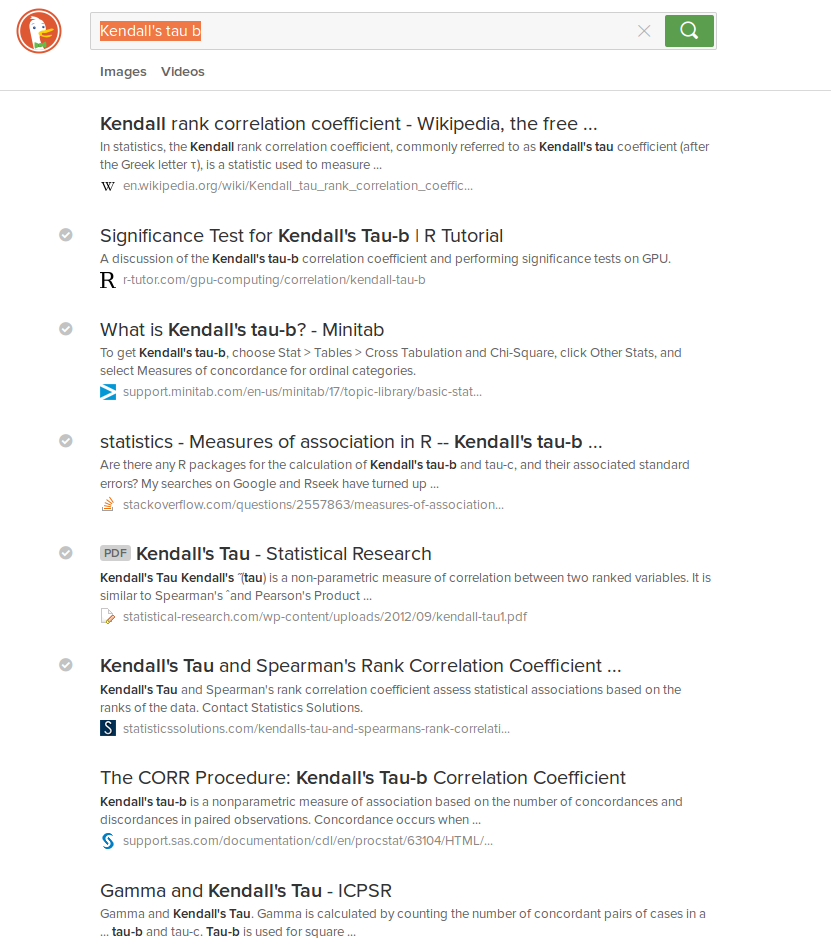
\includegraphics[scale=0.5]{KendallTauSearch.png}
	\caption{Kendall's tau b search}
    \label{fig:searchktb}
\end{figure}



 
\clearpage
\bibliographystyle{acm}
\bibliography{references}        
\end{document}